\chapter{Extended Cavity Diode Laser (ECDL)}\label{ECDL}
	\section{Introduction to LD tuning}
The light emitted by a diode laser greatly diverges in an oval shape pattern. Such a wide beam is practically useless to an experimentalist. Therefore, it is necessary to collimate the output of the diode laser, that is, bend the diverging light through a lens (or several lenses) so that all the output goes in one direction. One can achieve this result using a single lens as long as the laser is placed exactly at the focal  point of the lens one chooses. The focal point of a lens is also the point through which all light parallel to its normal axis will converge. Hence, if we place our diode laser at the focal point of our collimating lens all light from the diode laser that passes through the lens will exit parallel to the normal axis and all light that enters the face of the lens at normal incidence will be focused the diode laser. This property of optics allows us to send optical feedback back into the laser. Because of its small cavity, diode lasers have a large bandwidth, which means that the laser emits light over a broader range of wavelengths than other lasers. 

The broad linewidth of solitary diode laser often reduces their usefulness for spectroscopy applications. To overcome this problem several techniques have been developed, for example:
\begin{enumerate}
\item negative electronic feedback
\item resonant optical feedback from a high-finesse optical cavity
\item extended-cavity configurations
\end{enumerate}
Among all these techniques that can be used to reduce the laser linewidth down to the kHz range, the extended-cavity configuration with grating feedback has become the most popular. It provides a simple mean to achieve a wide wavelength tuning range and a narrow linewidth.
Several reasons, why we need to construct good external cavity:
\begin{enumerate}
\item an external cavity is capable of producing very short, sharp pulse in the range of picoseconds by means of mode-locking.
\item the external cavity provides high modal stability through optical feedback; mode hoping is several reduced.
\item a very narrow linewidth can be obtained by coupling a laser diode to an external cavity.
\end{enumerate}
There are 3 cavities which set up in experiments:
\begin{enumerate}
\item Laser diode cavity or internal Fabry-P\'{e}rot cavity
\item External cavity between grating and back side of the diode 
\item Parasitic cavity between grating and the front facet of the diode
\end{enumerate}

One of the ways to narrow the bandwidth of a diode laser is to use optical feedback to drive the laser at a single allowed lasing frequency. The collimation lens of the ECDL (Extended Cavity Diode Laser) is one critical part of attaining optical feedback. The second part of our system that allows optical feedback is the diffraction  grating. 

	\section{Diffraction theory for a grating}\label{gratingtheory}
A diffraction grating is a finely scored reflective material that, due to its geometry, allows only certain wavelengths of light incident at an angle $\theta$ to interfere constructively with itself as it is reflected outwards. The formula for constructively diffracted orders of light reflected from a diffraction grating is:
\mate
d\sin\theta=m\lambda
\atem
where $d$ is the spacing between reflective surfaces, $\theta$ is the angle of incidence, $\lambda$ is the wavelength of the incident light and $m$ is an integer. One consequence of the above equation is that spectra diffracted off a grating are reproduced at several different angular positions about the grating. The various replications of the spectra are called \textit{orders of diffraction} and obey the following relationship 
\mate
\sin\theta_{\mai{i}} + \sin\theta_{\mai{m}}= N m \lambda
\atem
where $\theta_{\mai{m}}$ is the angle of the $m$th order diffracted beam, $N$ is the spatial frequency of the grating (units mm$^{-1}$), and $\theta_{\mai{i}}$ and $\lambda$ are the incident light angle and wavelength respectively.

A schematic layout of the extended-cavity laser is outlined in \cref{grating}. The laser system consists of a diode laser as the active medium, a collimating lens and a diffraction grating. The external cavity is formed between the rear facet of the diode laser and the grating as a wavelength selective mirror. The laser frequency depends critically on the optical length of the cavity, which is sensitive to any changes in the refractive index of the cavity media (diode laser, lens, and air) and to changes in the physical cavity length.

\begin{figure}[!hbt]\centering
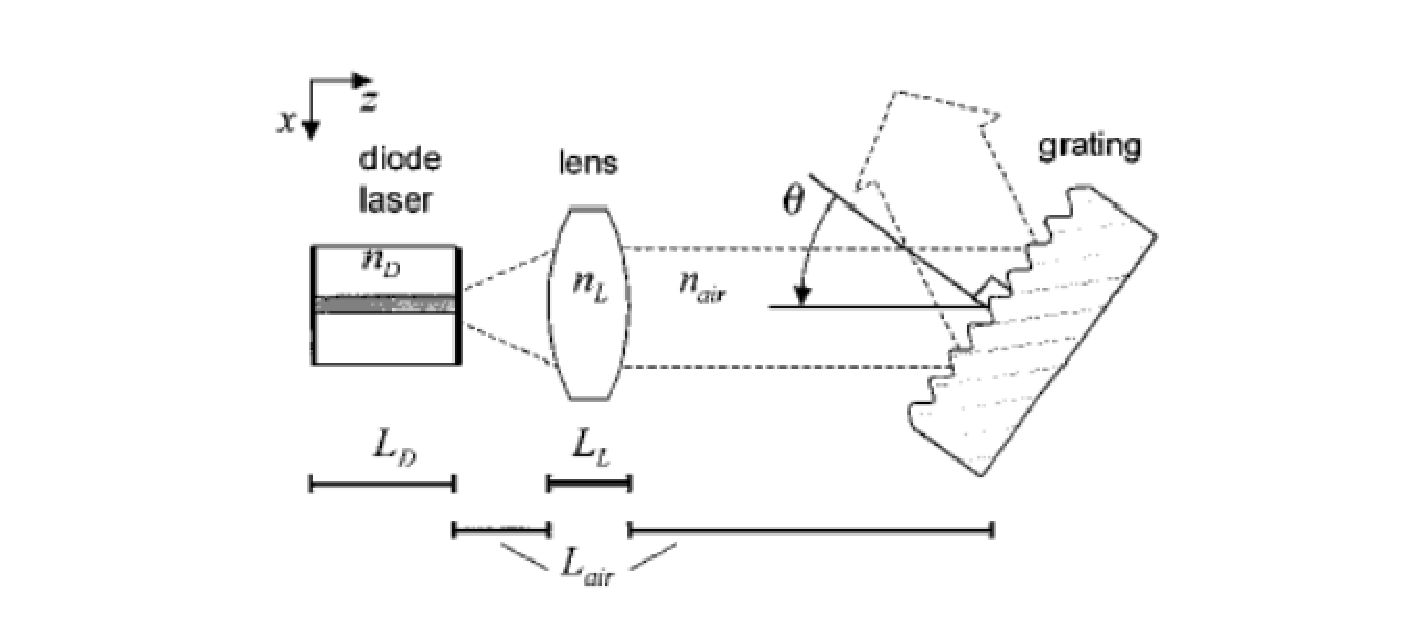
\includegraphics[width=\linewidth, draft=\foto]{eps/littrow1.eps}
\caption{Schematic layout of the extended cavity laser. The total optical path length in the cavity is $L_{\mai{ec}}=L_{\mai{d}}n_{\mai{d}}+L_{\mai{l}}n_{\mai{l}}+L_{\mai{air}}n_{\mai{air}}$}
\label{grating}
\end{figure}

	\section{Littrow configuration ECDL}\label{Littrowsection}
In the Littrow configuration for the external cavity, shown in \cref{littrow2}, the grating is aligned in way such that the first order diffraction from the grating is coupled directly back into the laser, while the zeroth-order diffraction is reflected as the output beam. The lasing wavelength is dependent on the angle of the incident laser beam with respect to the grating, otherwise known as the Littrow angle $\theta$.

\begin{figure}[!t]
\centering
%\mbox{
%\begin{minipage}[b]{.60\textwidth}
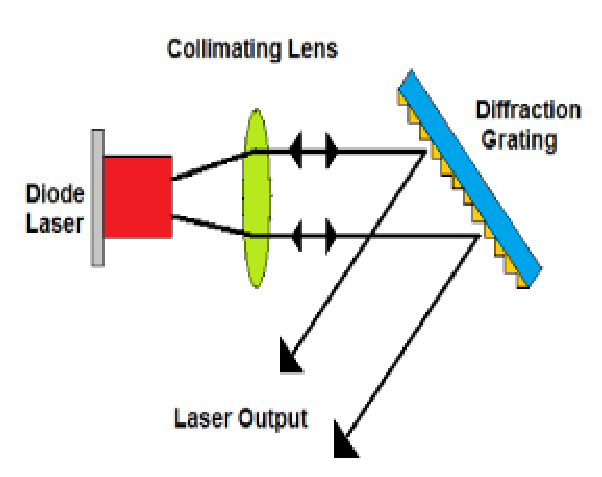
\includegraphics[width=0.7\linewidth, height=5cm, draft=\foto]{eps/littrow2.eps}
%\end{minipage}
%\begin{minipage}[b]{.35\textwidth}
\caption{Schematic diagram of external cavity in Littrow configuration.}
\label{littrow2}
%\end{minipage}}
\end{figure}

The key to the Littrow configuration is the backcoupling of the first-order diffraction beam from the grating into the laser diode. Without this feedback, the Littrow laser cannot achieve single-mode emission and will lase at a wavelength set by the gain peak of the semiconductor active region. When the feedback beam is well aligned, interference fringes are expected in the output beam and the laser remains in single-mode despite small temperature and current changes.

When monochromatic light impinges on a grating surface, it is diffracted into discrete directions. The light diffracted by each groove combines to form a diffracted wavefront. Diffraction by a grating can be visualized from the geometry in \cref{littrow4}, which shows a light ray of wavelength $\lambda$ incident at an angle $\alpha$ and diffracted by a grating along angles $\beta_{\mai{m}}$. These angles are measured from the grating normal, which is the dashed line perpendicular to the grating surface at its center. The sign convention for these angles depends on whether the light is diffracted on the same side or the opposite side of the grating as the incident light. In \cref{littrow3a}, which shows a reflection grating, the angles are  $\alpha>0$ and $\beta_{\mai{1}}>0$ (since they are measured counter-clockwise from the grating normal), while we have $\beta_{\mai{0}}<0$ and $\beta_{\mai{-1}}<0$ (since they are measured clockwise from the grating normal). Diagram \cref{littrow3b} shows the case for a transmission grating.
\begin{figure}[!bht]\centering
\subfigure[A reflection grating: the incident and diffracted rays lie on the same side of the grating.\label{littrow3a}]{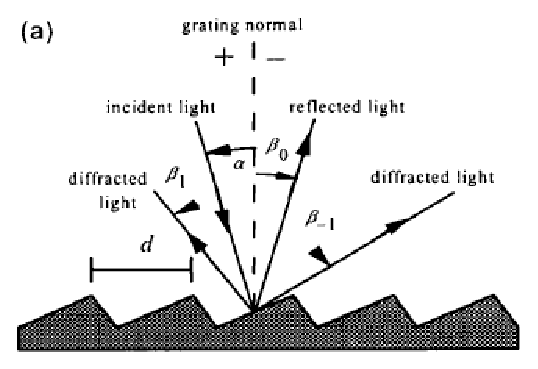
\includegraphics[width=.46\linewidth, draft=\foto]{eps/littrow3a.eps}}
\hfill
\subfigure[A transmission grating: the incident and diffracted rays lies on opposite sides of the grating.\label{littrow3b}]{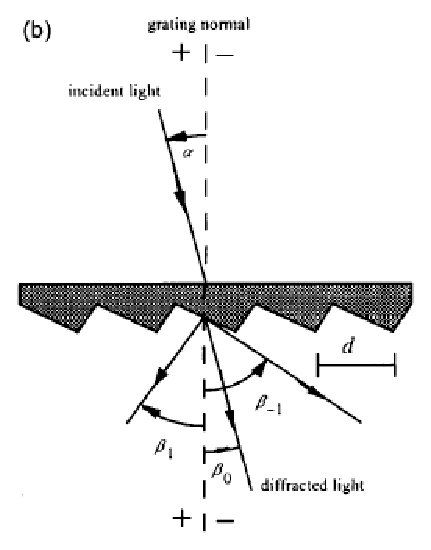
\includegraphics[width=.46\linewidth, draft=\foto]{eps/littrow3b.eps}}
\caption{A comparison between reflection and transmission grating.}
\end{figure}
For a grating of groove spacing $d$, there is a purely mathematical relationship between the wavelength and the angles of incident and diffraction. In a given spectral order $m$, the different wavelengths of polychromatic wavefronts incident at angle $\alpha$ (\cref{littrow4}) are separated in angle:
\mate
\beta[\lambda]=\arcsin\left[\frac{m\lambda}{d} – \sin\alpha\right]
\atem
When $m=0$, the grating acts as a mirror, and the wavelengths are not separated ($\beta=-\alpha$ for all $\lambda$); this is called specular reflection or \textit{the zeroth order}. 

The case in which the light is diffracted back towards the direction from which it came ($\alpha=\beta$) is called the \textit{Littrow configuration}. The grating equation is then given by
\mate
M\lambda=2d\sin\alpha
\atem
\begin{figure}[!htb]\centering
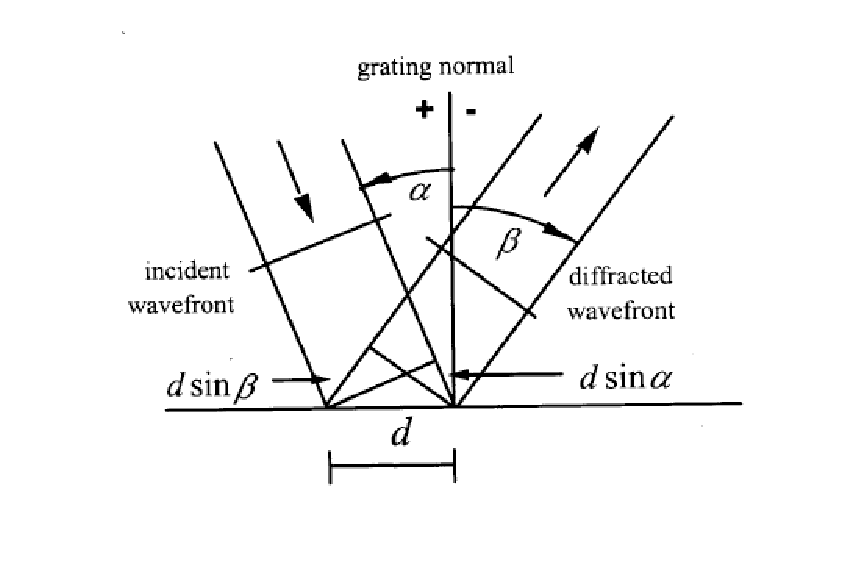
\includegraphics[width=\linewidth, draft=\foto]{eps/littrow4.eps}
\caption{Geometry of diffraction, for planar wavefronts.}
\label{littrow4}
\end{figure}

	\section{Main sources of noise in a ECDL}
The frequency of a solitary diode laser is sensitive to variations in the injection current and the junction temperature. This is mainly caused by changes in the refractive index of the active medium.

The optical length of the collimating lens changes with temperature. This is caused by thermal expansion of the material and temperature dependence of the refractive index. Their effects on the laser frequency are described by the relationship 
\mate
\frac{d\nu}{dT_{\mai{l}}}=-\nu\frac{L_{\mai{l}}}{L_{\mai{ec}}}\alpha_{\mai{l}}\left(n_{\mai{l}}-n_{\mai{air}}+\beta_{\mai{l}}n_{\mai{l}}\right)
\label{effect1}
\atem
where $n_{\mai{l}}$ and $n_{\mai{air}}$ are the refractive indices of the lens material and air respectively, and $L_{\mai{l}}$ and $L_{\mai{ec}}$ are the physical length of the lens and the total optical path length of the external cavity, respectively. The thermal expansion coefficient of the lens material is denoted by $\alpha_{\mai{l}}$ and the relative temperature coefficient of the refractive index by $\beta_{\mai{l}}$. 

The refractive index of air is mainly sensitive to variations in pressure $p$ and temperature $T_{\mai{air}}$.The variations in the laser frequency due to these changes are described by
\begin{align}
\frac{d\nu}{dp}=-\nu\frac{L_{\mai{air}}}{L_{\mai{ec}}}\frac{dn_{\mai{air}}}{dp}\label{effect2}\\
\frac{d\nu}{dT_{\mai{air}}}=-\nu\frac{L_{\mai{air}}}{L_{\mai{ec}}}\frac{dn_{\mai{air}}}{dT_{\mai{air}}}
\label{effect3}
\end{align}
where $L_{\mai{air}}$ is the cavity length containing air.	

The mechanical structure of the cavity often contains micrometric screws and piezoelectric transducers (PZTs) for wavelength control. The sensitivity of the laser frequency to thermal expansion of these parts can be written as
\mate
\frac{d\nu}{dT_{\mai{m}}}=\pm\nu\frac{L_{\mai{m}}}{L_{\mai{ec}}}\alpha_{\mai{m}}
\label{effect4}
\atem
where $L_{\mai{m}}$ and $\alpha_{\mai{m}}$ are the length and the thermal expansion coefficient of the mechanical part, respectively.

A transverse displacement along $x$ axis of the collimating lens with respect to the laser diode changes the beam direction. This causes a frequency shift due to a change in the cavity length. For a small displacement, the frequency shift can be written as
\begin{align}
\frac{d\nu}{dx}=\frac{\nu\tan\theta}{f_{\mai{l}}}
\label{displacement}\\
\frac{d\nu_{\mai{g}}}{dT}=-\nu_{\mai{g}}\alpha_{\mai{g}}
\label{displacement2}
\end{align}
where $f_{\mai{l}}$ is the focal length of the lens and $\theta$ is the angle between the grating normal and the incident beam, while $\nu_{\mai{g}}$ and $\alpha_{\mai{g}}$ are the cental frequency of the grating feedback and the grating thermal expansion coefficient respectively. The displacement of the lens can be caused, for example, by asymmetric thermal expansion relative to the optical axis or by mechanical vibration of the lens holder. 

There are additional effects that influence mainly the short-term frequency stability of the laser: current- and PZT driver noise, mechanical vibrations, acoustic disturbances, and rapid changes in the refractive index of air caused by air flow. All of these factors have an effect on the length of the external cavity and, consequently, generate frequency modulation of the laser.
